\documentclass[journal,10pt,twocolumn]{article}
\usepackage[margin=0.5in]{geometry}
\usepackage[cmex10]{amsmath}
\usepackage{amsmath}
\usepackage{array}
\usepackage{booktabs}
% The preceding line is only needed to identify funding in the first footnote. If that is unneeded, please comment it out.
\usepackage{cite}
\usepackage{amsmath,amssymb,amsfonts}
\usepackage{graphicx}
\usepackage{textcomp}
\usepackage{xcolor}
\graphicspath{{./figs/}}{}
\usepackage{amsmath,amssymb,amsfonts,amsthm}
\usepackage{gensymb}
\newcommand{\myvec}[1]{\ensuremath{\begin{pmatrix}#1\end{pmatrix}}}
\let\vec\mathbf
\title{
Optimization-Assignment
}
\author{SHREYASH CHANDRA PUTTA}
\providecommand{\norm}[1]{\left\lVert#1\right\rVert}
\providecommand{\abs}[1]{\left\vert#1\right\vert}
\let\vec\mathbf
\newcommand{\mydet}[1]{\ensuremath{\begin{vmatrix}#1\end{vmatrix}}}
\providecommand{\brak}[1]{\ensuremath{\left(#1\right)}}

\begin{document}
\maketitle
\tableofcontents
\bigskip
\section{Problem Statement}
If x and y are positive real numbers such that $x^2 +y^2 = 1$ then Find the maximum value of \textbf(x+y)

\section{Solution}

Given Problem can be expressed as 
\begin{align}
\label{eq:1}
\max_{\vec{x}}{\vec{n}}^T{\vec{x}}\\
\label{eq:2}
\text {s.t. }\vec{x}^T\vec{V}\vec{x} + \vec{u}^T\vec{x}  +d = 0
\end{align}
%
where
%
\begin{align}
\vec{V} &= \myvec{1 & 0\\0 & 1} or \vec{I}
\\
\vec{u} &= -\myvec{0 \\ 0}
\\
d &= -1
\\
\vec{n} &= \myvec{1 \\ 1}
\end{align}

%%%%%%%%%%%%%%%%%%%%%%%%%%%%%%%%%%%%%%%%%%%%%
the following relaxation makes
\eqref{eq:1} a convex optimization 

\begin{align}
\label{eq:7}
\max_{\vec{x}}\brak{\vec{n}}^T{\vec{x}}\\
\text{s.t. }\vec{x}^T\vec{V}\vec{x} + \vec{u}^T\vec{x} + d \le 0
\end{align}
%%%
Solve \eqref{eq:1} using cvxpy.
\\
The following code yields the maximum value of given condtion for the point on the curve as
%
{\setlength\extrarowheight{0pt}
\begin{table}[h]
    \centering
    \begin{tabular}{|c|}
    \hline \\
         https://github.com/chanduputta/\\FWC-Module1Assignments/blob/\\main/optimization/cvxopt.py  \\       
\hline
    \end{tabular}
\end{table}}
%
\begin{align}
\vec{Q} &= \myvec{1.4142\\1.4142}
\end{align}
from 
\begin{align}
\boxed{\text{Maximum value} = 1.4142 \approx \sqrt{2}} 
\end{align}

\subsection{verification} Graphically verify the solution to . 
by drawing a figure.
\\
The above code plots Fig. of given curve
%	

%
\begin{figure}[!ht]
\centering
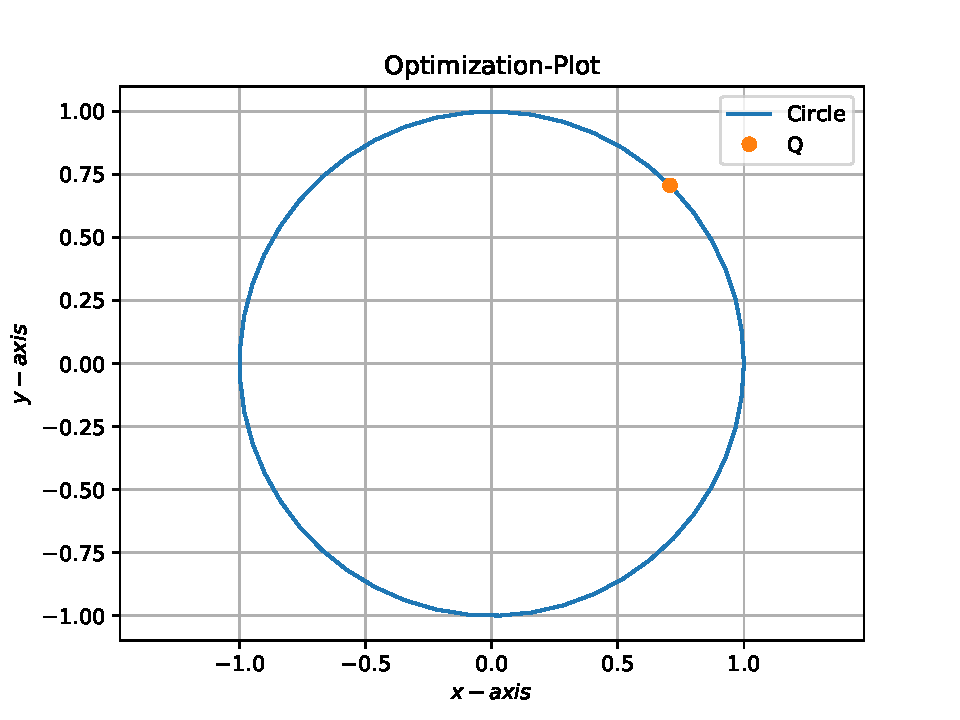
\includegraphics[width=\columnwidth]{fig/cvxoptfig.pdf}
\caption{ at $\vec{Q}$ the $\eqref{eq:1}$ gives $\sqrt{2}$ which is maximum }.
\label{fig:qp_parab}
\end{figure}

%%%%%%%%%%%%%%%%%%%%%%%%%%%%%%%%%%%%%%%%%%%%%%%%%%%%%%%%%%%

\end{document}
